\chapter*{标题一}
\addcontentsline{toc}{chapter}{标题一}

\section{小节标题 C\#}

这是一个\textbf{加粗}和\textit{斜体}的文本。

这里是一个链接:\href{https://www.google.com}{Google}

我们引用了一些文献\cite{foo},还有公式:$E = mc^2$

\texttt{Code \{ Rust \}} 是正常的吗,\texttt{foo\_bar} 呢?

\begin{lstlisting}
bool foo = true;
#define BLOCK_LIST "Block List, 'Block List'^{}";
\end{lstlisting}

\input{}
\begin{tabularx}{\textwidth}{|>{\centering\arraybackslash}X|>{\centering\arraybackslash}X|>{\centering\arraybackslash}X|>{\centering\arraybackslash}X|} \hline
名称 & 字段名 & 类型与范围 & 描述 \\ \hline
基础色贴图 & base\_color\_texture & 可选贴图 & 一个物体的基本颜色的贴图,用顶点(片源)的 UV 采样,长文本测试长文本测试长文本测试长文本测试长文本测试长文本测试 \\ \hline
法线贴图 & normal\_texture & 可选贴图 & 存储法线信息的贴图,用顶点(片源)的 UV 采样 \\ \hline
颜色 & color & [f32; 4] & 会与基础色贴图相乘 \\ \hline
粗糙度 & roughness & f32 [0.0~1.0] & 影响材质的粗糙感的参数,参与微表面模型的计算 \\ \hline
金属度 & metallic & f32 [0.0~1.0] & 影响材质的金属感的参数,参与微表面模型的计算 \\ \hline
反射度 & reflectance & f32 [0.0~1.0] & 影响材质的高光强度的参数,参与微表面模型的计算 \\ \hline
Alpha 模式 & alpha\_mode & 枚举:不透明、蒙板、混合 & 决定物体渲染方式的参数 \\ \hline
\end{tabularx}

C\# 啊啊啊

段落结束。

\begin{itemize}
\item 无序列表
\item 无序列表是无序号的
\item 无序列表是个列表
\end{itemize}
\begin{enumerate}
\item 有序列表
\item 有序列表是有序号的
\item 有序列表是个列表
\end{enumerate}
\begin{figure}[h]
\centering
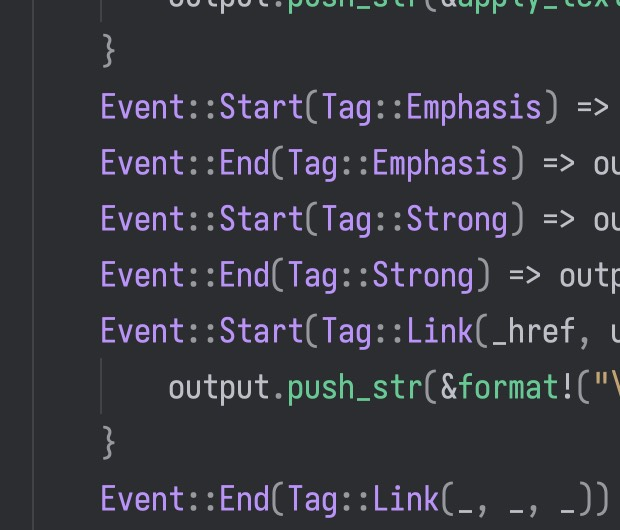
\includegraphics[width=0.8\textwidth]{images/test.jpg}
\caption{test image}
\label{fig:images/test.jpg}
\end{figure}


\begin{equation}
\label{eq:hhhhh}
\frac{1}{2}\mu
\end{equation}

